%%%%%%%%%%%%%%%%%%%%%%%%%%%%%%%%%%%%%%%%%%%%%%%%%%%%%%%%%%%%%%%%%%%%%%%%%%%%%%
\section{Evaluation}\label{sec:casper-eva}
%%%%%%%%%%%%%%%%%%%%%%%%%%%%%%%%%%%%%%%%%%%%%%%%%%%%%%%%%%%%%%%%%%%%%%%%%%%%%%

In this section, we evaluate Casper on two platforms: the NERSC Edison
Cray XC30 supercomputer
(https://www.nersc.gov/users/computational-systems/edison/configuration/)
and the Argonne Fusion cluster
(http://www.lcrc.anl.gov/about/fusion).  We used these two platforms
to demonstrate the impact of varying levels of hardware support for
RMA operations.  Specifically, Cray MPI (version 6.3.1) can be
executed in two modes: regular or DMAPP-based.  The regular version
executes all RMA operations in software with asynchronous progress
possible through a background thread.  The DMAPP version executes
contiguous PUTs and GETs in hardware, but accumulates and
noncontiguous operations are executed in software with asynchronous
progress through interrupts.  On the Fusion platform, we used
MVAPICH.  MVAPICH (version
2.0rc1\footnote{We had to fix a bug in MVAPICH to allow for true
  hardware-based RMA for PUT and GET.}) implements contiguous PUT/GET
operations in hardware, while using software active messages for
accumulates and noncontiguous operations (asynchronous progress using
a background thread).
% MPICH-SHM (git master from Sep. 23rd, 2014)
% implements all operations ``in hardware'' (i.e., on CPU instructions
% on the target).

We expect Casper to improve asynchronous progress in the cases where
RMA operations are implemented as \emph{software active messages} and
to perform as well as the original MPI implementation when hardware
direct RMA is used.
%GWP - note that you say performs - did you mean that it currently does perform equally well?
% Comment: yes.

%% Our experiments first focus on following three major aspects by
%% evaluating various microbenchmarks: (1)~analysis of the overheads
%% caused by Casper complex design for guaranteeing correctness; (2)~the
%% improvement of asynchronous progress with comparison to
%% other asynchronous progress approaches (an interrupt-based
%% asynchronous progress called DMAPP and MPICH asynchronous thread on
%% Cray X30; and MPICH asynchronous thread on InfiniBand cluster);
%% (3)~discussion of load balancing performance optimization.
%% After above deep analysis, we evaluate Casper by employing a real
%% computational chemistry application suite.

% \begin{table}\scriptsize
% \begin{center}
% \caption{MPI RMA implementations.}\label{tab:eva-mpi-rma}
% \begin{tabular}{|c|c|}
% \hline
% Cray MPI & AM \\
% Mvapich & AM + direct RMA \\
% MPICH-SHM & direct RMA \\
% \hline
% % \multicolumn{2}{p{3.0cm}|}{} \\
% % \hline
% \end{tabular}
% \end{center}
% \begin{center}
% \begin{minipage}{8.0cm}
% \footnotesize{Note. AM means Active Message, the software
% implementation of RMA; Direct RMA mean hardware RMA.}
% \end{minipage}
% \end{center}
% \end{table}


%%%%%%%%%%%%%%%%%%%%%%%%%%%%%%%%%%%%%%%%%%%%%%%%%%%%
\subsection{Overhead Analysis}\label{sec:eva-overhead}
%%%%%%%%%%%%%%%%%%%%%%%%%%%%%%%%%%%%%%%%%%%%%%%%%%%%

In this section, we measure two overheads caused by Casper: (1) window
allocation and (2) Fence and PSCW.

As discussed in Section~\ref{sec:des-init}, Casper internally creates
additional overlapping windows in order to manage lock permissions
when a ghost process supports multiple user processes.  These can cause
performance overhead.  However, the amount of overhead can be
controlled by setting the info argument \texttt{epoch\_type} to tell
Casper which epoch types are used by the application.  Accordingly
Casper can decide which internal windows it needs to create.
Figure~\ref{fig:eva-cray-overh-win-alloc} shows the overhead of
\fn{MPI\_WIN\_ALLOCATE} on a user process with varying total numbers of
processes on a single node of Cray XC30. When no info hints
are passed (default \texttt{epoch\_type} is ``fence,pscw,lockall,lock''),
Casper can experience substantial performance cost in window creation time.
When \texttt{epoch\_type} is set to ``lock,'' Casper does not have to
create the additional window for active target and lockall
communication, thus improving performance a little; but the cost is
still considerable because Casper has to create one window for every user process
on that node.  When \texttt{epoch\_type} is set to ``lockall'' or
``fence'' (or any other value that does not include ``lock''), Casper
has to create just one additional internal window, thus reducing the
cost substantially, although the cost is still more than twice that of
original MPI.

The second major overhead occurs because of the conversion of fence and
PSCW to passive-target epochs and the additional synchronization and
memory consistency associated with it. We measure these overheads by
using two interconnected processes on Cray XC30.
The fence experiment performs \emph{fence--accumulate--fence} on the first
process and \emph{fence--fence} on the other, with the first passing
the \texttt{MPI\_MODE\_NOPRECEDE} assert and the second fence passing
the \texttt{MPI\_MODE\_NOSUCCEED} assert.  The PSCW experiment
performs \emph{start--accumulate--complete} and \emph{post--wait} on
the two processes. Figure~\ref{fig:eva-cray-overh-active} shows
the execution time of our experiments on the first process. While the
overhead is large (100--200\%) for a small number of operations, as the
number of operations issued increases, this cost gets amortized and disappears.

% \parahead{Self Lock.}
% As we have described in Section~\ref{sec:self-lock},
% Casper issues a \emph{get-flush} and a second \emph{self-lock}
% for guaranteeing the lock permission correctness and memory consistency,
% resulting in additional overhead.
% Two user hints could reduce above overhead:
% \textit{MPI\_MODE\_NOCHECK} assert eliminates the first step but
% still requires the second one for memory consistency of local
% load\slash store; \textit{no\_local\_load\_store} info eliminates
% both steps because neither lock permission nor local memory
% consistency need to be maintained in this case.
% Figure~\ref{fig:eva-overh-lockself} compares the overhead of
% self lock on both Cray XC30 and on a shared node of InfiniBand cluster
% using MPICH-SHM. We measure a simple \emph{lock(self)-put(self)-unlock(self)}
% microbenchmark with one application process.
% As shown in this figure, the default self lock always produces
% the heaviest overhead, 1~$\mu$s on InfiniBand cluster and
% 1.4~$\mu$s on Cray respectively. On InfiniBand node, the lock with
% \textit{no\_local\_load\_store} performs the smallest overhead;
% the \textit{NOCHECK} does not reduce overhead much
% because the additional \emph{get-flush} does not have much overhead
% on a shared memory node in which RMA operations are performed as
% direct RMA but the overhead of memory barrier become dominant.
% However, we get different trend on Cray, because Cray MPI still
% performs RMA operations as remote AM in shared memory node if
% the window is created by \textit{MPI\_WIN\_CREATE} which degrades
% local RMA performance and we translate these RMA operations
% to the process itself if lock is acquired (as in default lock and
% \textit{NOCHECK}) as a workaround. This is the reason why
% \textit{NOCHECK} assert delivers the most performance improvement.

% \parahead{(3). RMA operation redirection}

% After shows the overhead for synchronization calls, we also measured
% the additional overhead of RMA operations caused by the translation
% and load balancing processing as shown in Figure~\ref{fig:eva-mxm-overh-op-shm}
% , \ref{fig:eva-cray-overh-op-inter}, \ref{fig:eva-mxm-overh-op-shm}
% and \ref{fig:eva-cray-overh-op-inter}. Roughly speaking, the
% overhead of each RMA operation are alway a constant value lower than
% 1~$\mu$s and can be ignored with increasing of operation size or
% the delay caused by user computation. \textcolor{red}{[why internode
% overhead is constant percentage ? ]}

% The third overhead of Casper comes from the RMA operation
% segmentation. As we have discussed in Section~\ref{sec:multi-ghost},
% when multiple ghost processes exist in the system, we need
% static binding for lock permission correctness.
% \textit{Static Segment Binding} is one of the
% solutions to overcome the permission issue, but with additional
% overhead. We demonstrate such overhead using a simple microbenchmark
% with two interconnected processes. Every process first allocates a
% large window which will be divided to several segments
% and bound to different local ghosts; then when rank 0 issues a large
% ACCUMULATE to rank 1, such operation will be divided to multiple
% operations if the data contains multiple segments. We specify
% the window size is 1024 count of double, thus it will be divided
% to two 512 count of double segments with 2 ghost processes, four 256
% count of double segments with 4 ghost processes, and eight 128 count
% of double segments with 8 ghost processes. As shown in Figure~
% \ref{fig:eva-cray-overh-op-seg}, when ACCUMULATE size is 128, which
% is always smaller than the segment size, there is not much overhead
% with increasing of ghosts. However, for a 256 and 512 count of
% double ACCUMULATE, significant overhead occurs with increasing of
% ghosts processes because more operations have to be produced internally.



\begin{figure}
\centering
\subfigure[Window allocation overhead.]{
  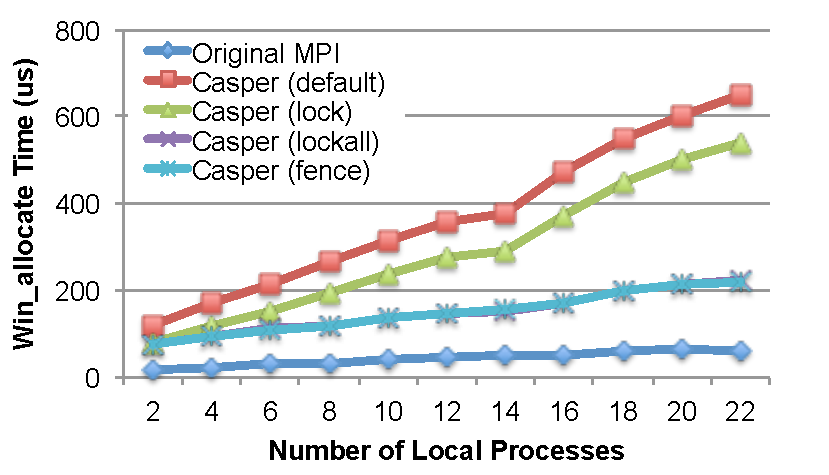
\includegraphics[width=0.85\columnwidth]{figures/casper/eva_edison_overhead_win_alloc.pdf}
  \label{fig:eva-cray-overh-win-alloc}
}
\subfigure[Fence and PSCW overhead]{
  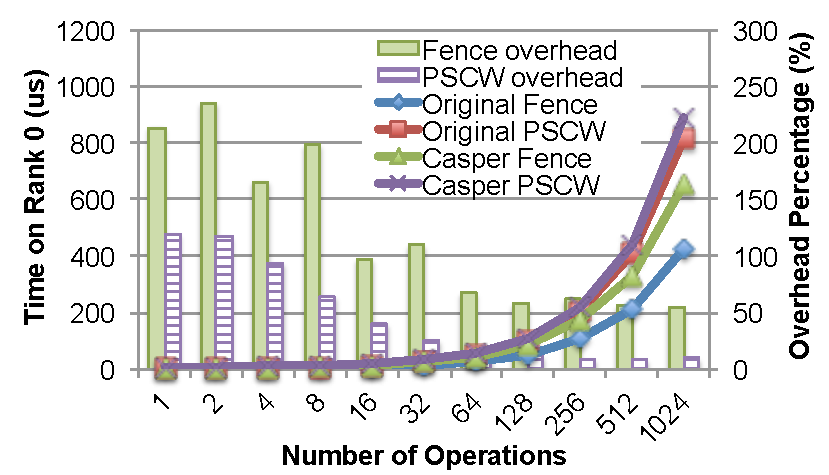
\includegraphics[width=0.85\columnwidth]{figures/casper/eva_edison_overhead_fence_pscw.pdf}
  \label{fig:eva-cray-overh-active}
}
% \subfigure[RMA operation segmentation]{
%   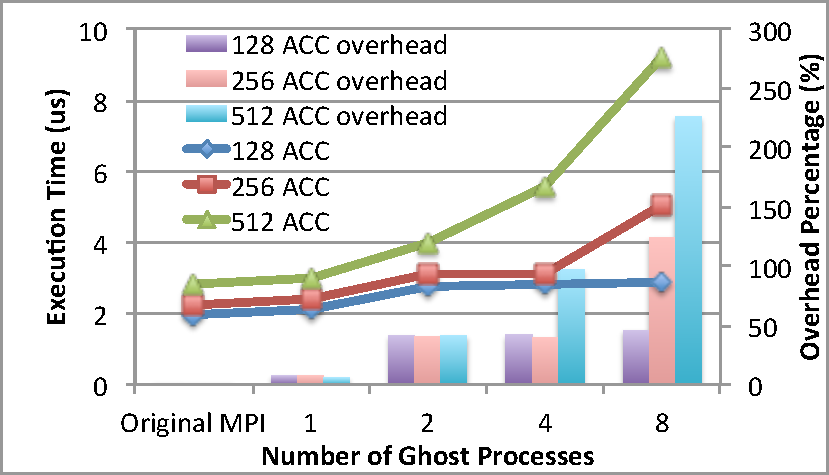
\includegraphics[width=0.62\columnwidth]{figures/casper/eva_cray_overhead_op_seg.pdf}
%   \label{fig:eva-cray-overh-op-seg}
% }
% \subfigure[Overhead when locking process itself on InfiniBand using MPICH-MXM.]{
%   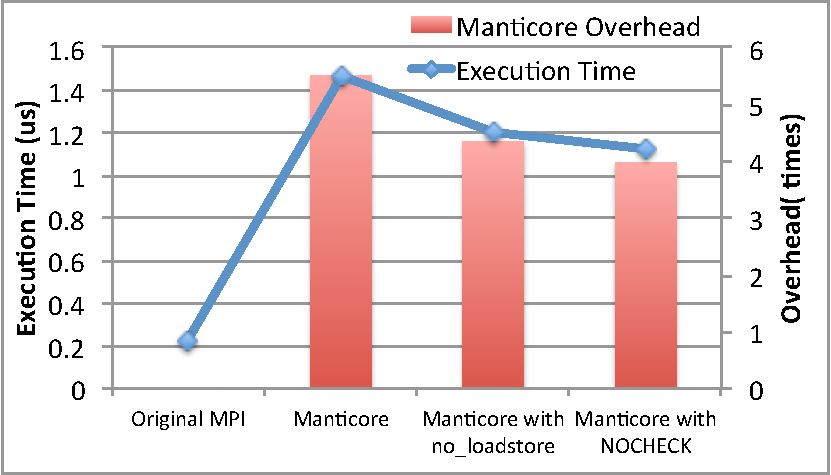
\includegraphics[width=0.63\columnwidth]{figures/casper/eva_mxm_overhead_lockself.pdf}
%   \label{fig:eva-mxm-overh-lockself}
% }
% \subfigure[Overhead of SHM RMA operation redirection on InfiniBand using MPICH-MXM.]{
%   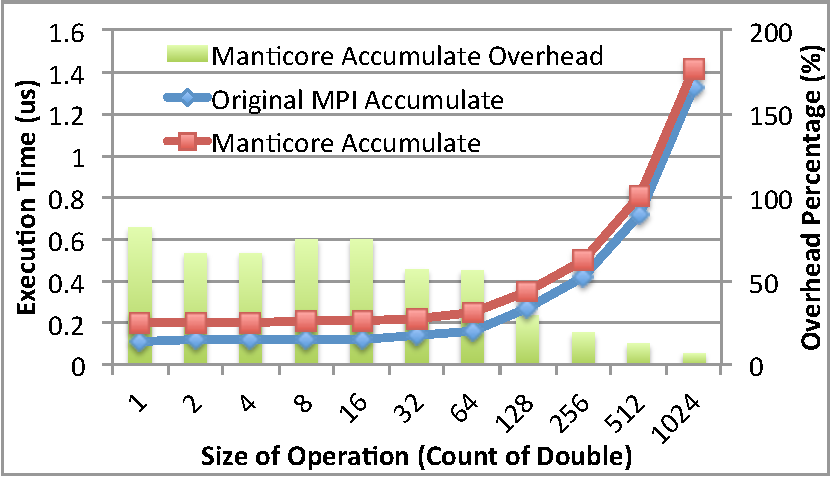
\includegraphics[width=0.63\columnwidth]{figures/casper/eva_mxm_overhead_op_shm.pdf}
%   \label{fig:eva-mxm-overh-op-shm}
% }
% \subfigure[Overhead of Inter-node RMA operation redirection]{
%   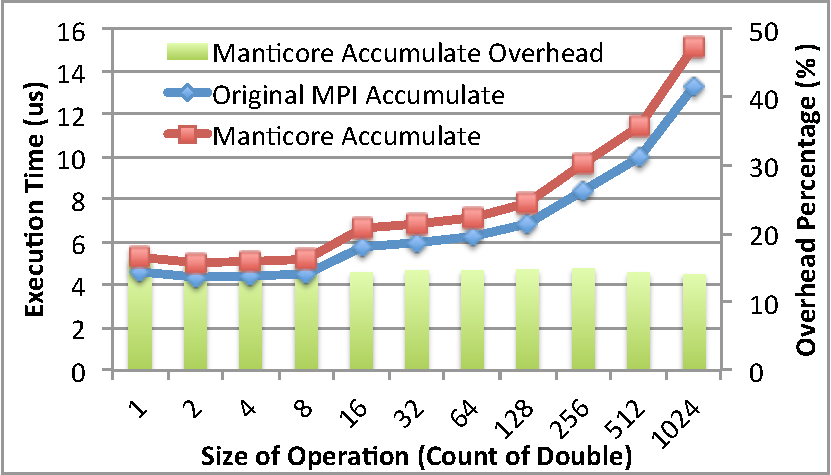
\includegraphics[width=0.63\columnwidth]{figures/casper/eva_mxm_overhead_op_inter.pdf}
%   \label{fig:eva-mxm-overh-op-inter}
% }
% \subfigure[Overhead of RMA operation segmentation]{
%   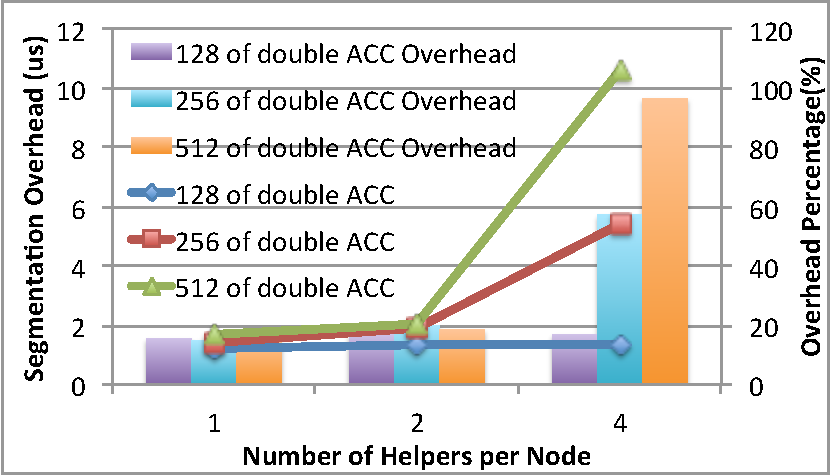
\includegraphics[width=0.63\columnwidth]{figures/casper/eva_mxm_overhead_op_seg.pdf}
%   \label{fig:eva-mxm-overh-op-seg}
% }
% \caption{Overhead Analysis on InfiniBand cluster using MPICH.}
% \footnotesize{\textcolor{red}{Why internode op overhead increase ? }}
% \label{fig:eva-mxm-overh}
% \end{figure*}
% \begin{figure*}
% \centering
% \subfigure[Lockall overhead on Cray X30.]{
%   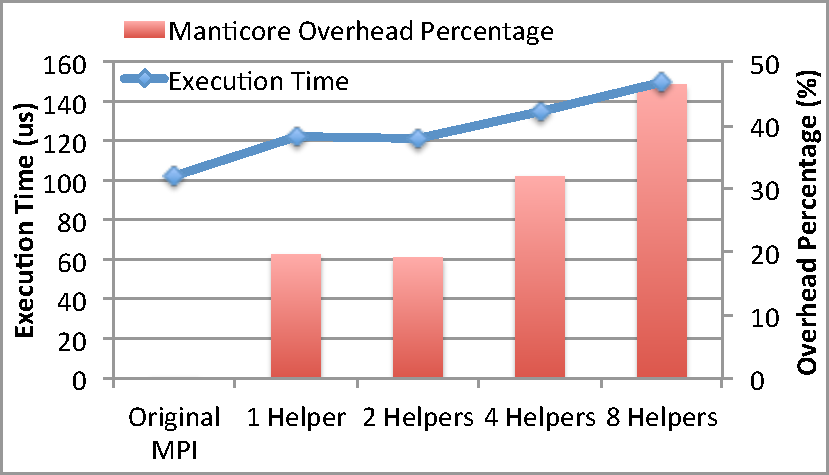
\includegraphics[width=0.63\columnwidth]{figures/casper/eva_cray_overhead_lockall.pdf}
%   \label{fig:eva-cray-overh-lockall}
% }
% \subfigure[Local lock]{
%   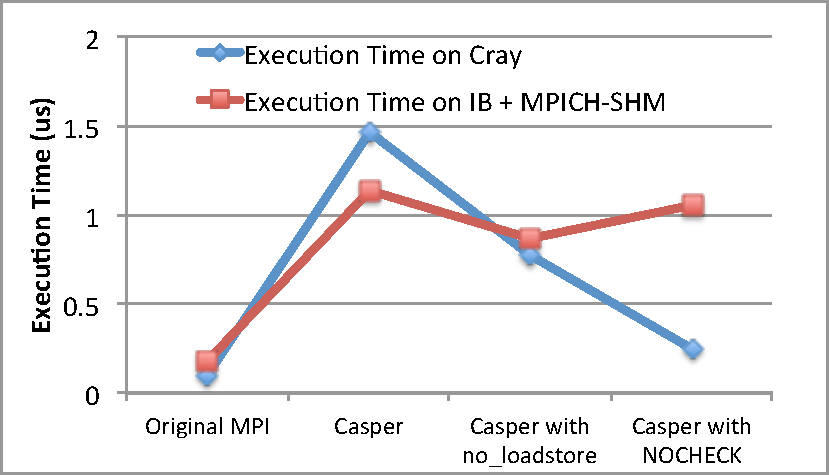
\includegraphics[width=0.63\columnwidth]{figures/casper/eva_overhead_lockself.pdf}
%   \label{fig:eva-overh-lockself}
% }
% \subfigure[Overhead of SHM RMA operation redirection on Cray X30.]{
%   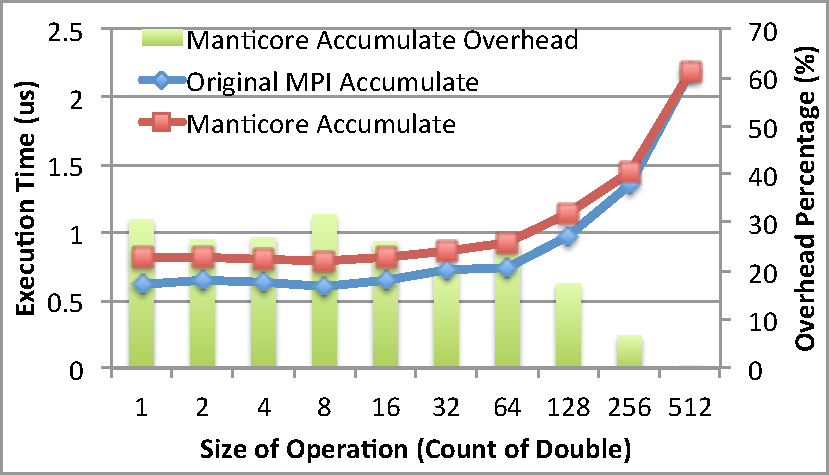
\includegraphics[width=0.63\columnwidth]{figures/casper/eva_cray_overhead_op_shm.pdf}
%   \label{fig:eva-cray-overh-op-shm}
% }
% \subfigure[Overhead of Inter-node RMA operation redirection]{
%   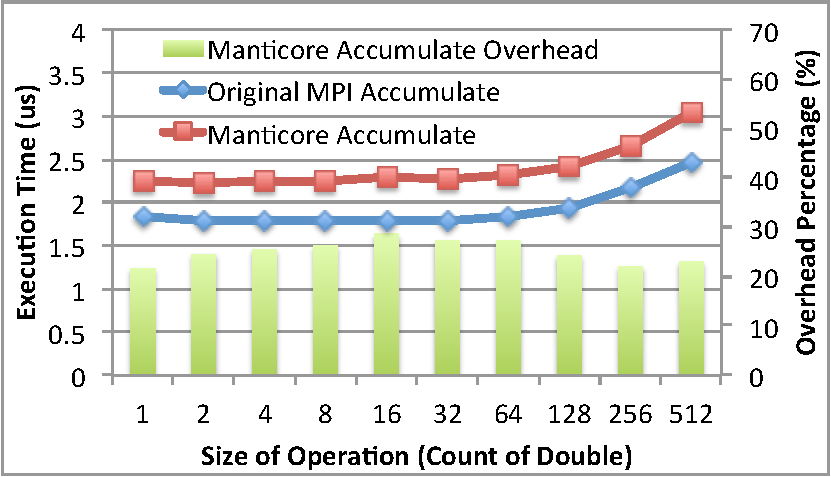
\includegraphics[width=0.63\columnwidth]{figures/casper/eva_cray_overhead_op_inter.pdf}
%   \label{fig:eva-cray-overh-op-inter}
% }
% \vspace{-1.5ex}
\caption{Overhead analysis.}
\label{fig:eva-cray-overh}
% \vspace{-4.0ex}
\end{figure}


%%%%%%%%%%%%%%%%%%%%%%%%%%%%%%%%%%%%%%%%%%%%%%%%%%%%
\subsection{Asynchronous Progress }\label{sec:eva-scala}
%%%%%%%%%%%%%%%%%%%%%%%%%%%%%%%%%%%%%%%%%%%%%%%%%%%%

In the section, we demonstrate the asynchronous progress improvements
achieved in various scenarios.

%%%%%%%%%%%%%%%%%%%%%%%%%%%%%%%%%%%%%%%%%%%%%%%%%%%%
\subsubsection{Different Synchronization Modes}\label{sec:eva-overlap}
%%%%%%%%%%%%%%%%%%%%%%%%%%%%%%%%%%%%%%%%%%%%%%%%%%%%

Our first experiment demonstrates the improvement of computation and
communication overlap in passive and active-target modes using Casper.
Two interconnected processes are used in each mode.  In
the passive-target mode, one process issues
\emph{lockall--accumulate--unlockall} to another process while that
process is blocking in computation.
Figure~\ref{fig:eva-cray-async-lockall} shows the results on
the Cray XC30.  As expected, with the original MPI the execution time
on the origin increases with wait time on the target, which means that the
origin is blocked by the computation on the target.  All asynchronous
progress approaches relieve this issue.  We note, however, that both
the DMAPP and thread approaches have more overhead than Casper does.

The overhead with using the MPICH asynchronous thread comes from the expensive
thread-multiple safety and lock contention.  DMAPP-based asynchronous
progress, however, does not involve thread-multiple safety and also
wakes up background threads only when a message arrives.  Therefore, to
analyze the reason for this overhead, we performed a test in which one
process does \emph{lockall--accumulate--unlockall} and the other
process does a \textit{dgemm} computation.  As shown in
Figure~\ref{fig:eva-cray-dmapp-overhead}, when we increase the number
of ACCUMULATEs issued in each iteration, DMAPP's overhead also
increases.  To further analyze this situation, we measured the number of system
interrupts. We found that they increased with the number of
ACCUMULATEs as well and were clearly becoming a bottleneck with
increasing numbers of operations.

% \begin{figure}[h]
% \begin{CenteredBox}
% \begin{lstlisting}[linewidth=0.73\columnwidth]
% MPI_Win_lock_all(win);
% if (rank == 0){
%     MPI_Accumulate(...);
%     MPI_Win_flush(1, win);
% }else{
%     while(MPI_Wtime() - start < WAIT_TIME);
%     MPI_Test(...);
% }
% MPI_Win_unlock_all(win);
% \end{lstlisting}
% \end{CenteredBox}
% \caption{Overlap improvement microbenchmark.}
% \label{code:test-src}
% \end{figure}

In the active-target mode, since both fence and PSCW require internal
synchronization in Casper, the origin has to wait for the completion
of the epoch on the target.  Thus, in an experiment similar to that for
the passive mode, we measured the time for
\emph{fence--accumulate--fence} on one process while another process
performs \emph{fence--100~$\mu$s busy waiting--fence} as shown in
Figure\ref{fig:eva-cray-async-fence}.  We notice that when a small
number of operations are issued during fence, asynchronous progress is
beneficial.  But when the communication takes more time than the delay
on the target, which is the maximum time Casper can overlap (larger
than 128 in the figure), the percentage improvement decreases, as
expected.  PSCW follows a similar trend. Both DMAPP and
thread asynchronous progress show significant overhead compared with that of the original
MPI execution.

\begin{figure*}
\centering
\subfigure[Passive-target RMA]{
  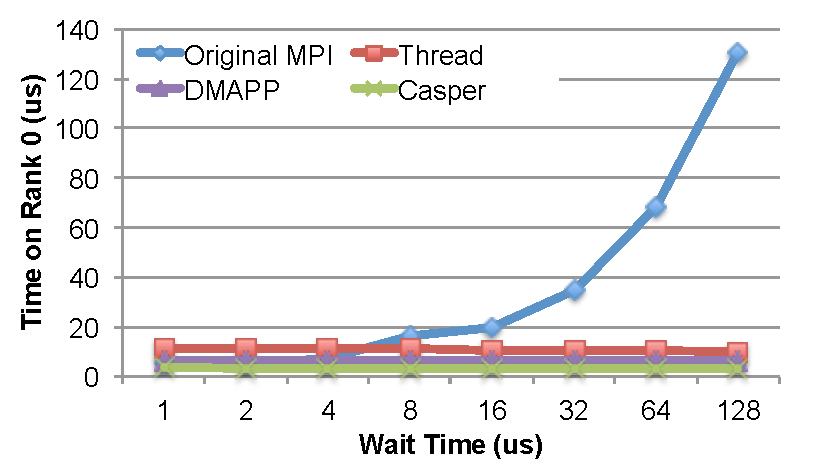
\includegraphics[width=0.64\columnwidth]{figures/casper/eva_cray_test2pe_s.pdf}
  \label{fig:eva-cray-async-lockall}
}
\subfigure[Fence RMA]{
  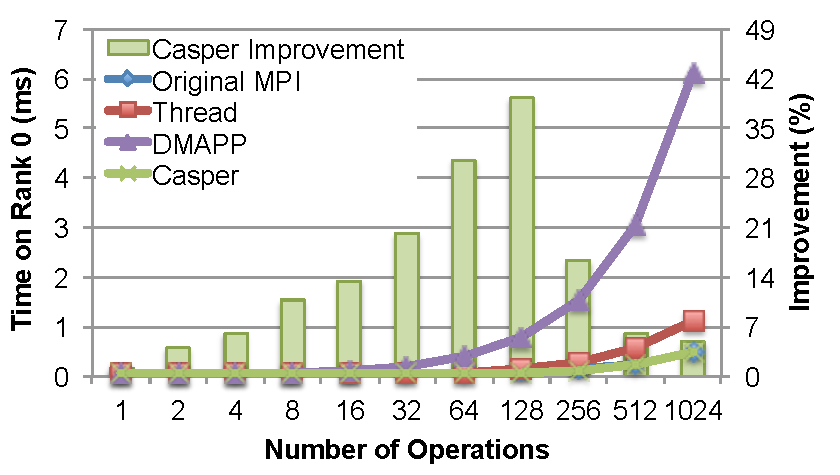
\includegraphics[width=0.64\columnwidth]{figures/casper/eva_cray_async_fence.pdf}
  \label{fig:eva-cray-async-fence}
}
\subfigure[Overhead of DMAPP interrupts]{
  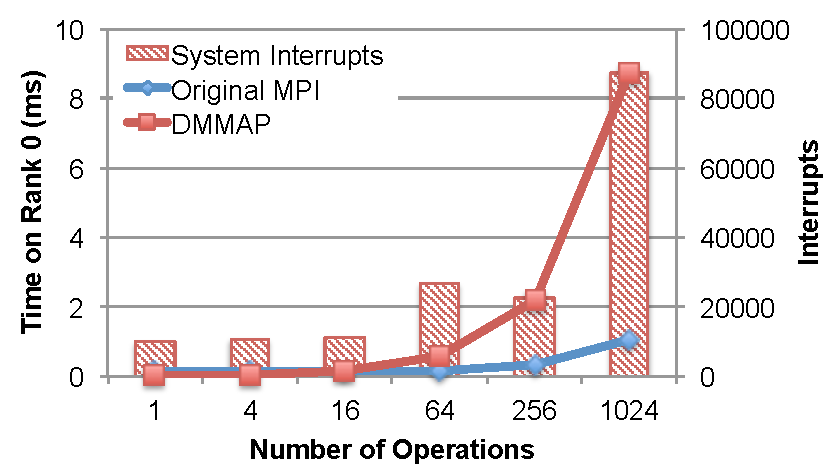
\includegraphics[width=0.64\columnwidth]{figures/casper/eva_cray_dmapp_overhead.pdf}
  \label{fig:eva-cray-dmapp-overhead}
}
% \subfigure[PSCW RMA\textcolor{blue}{[TODO]}]{
%   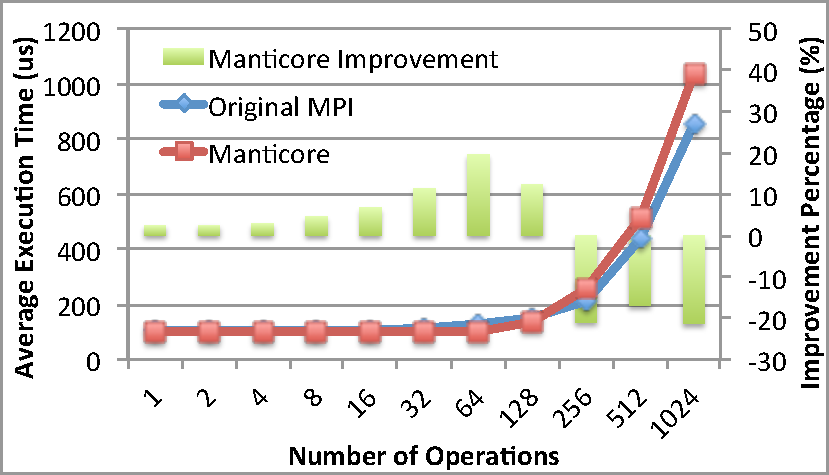
\includegraphics[width=0.63\columnwidth]{figures/casper/eva_cray_async_pscw.pdf}
%   \label{fig:eva-cray-async-pscw}
% }
% \vspace{-1.0ex}
\caption{Overlap improvement using two interconnected processes on
Cray XC30.}
\label{fig:eva-comm-overlap}
% \vspace{-4.0ex}
\end{figure*}


% \begin{figure}[h]
% \centering
% 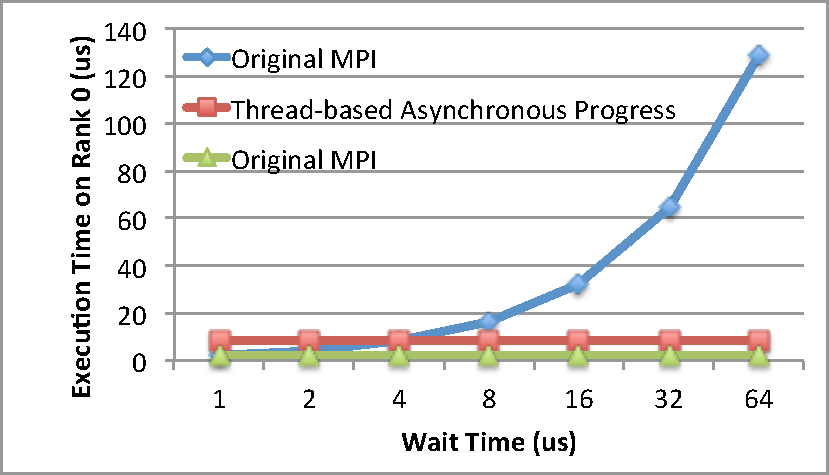
\includegraphics[width=0.8\columnwidth]{figures/casper/eva_fusion_lockall_shm_np2.pdf}
% \caption{Lockall asynchronism improvement using two processes on
% a shared memory node using MPICH-SHM.}
% \end{figure}

%%%%%%%%%%%%%%%%%%%%%%%%%%%%%%%%%%%%%%%%%%%%%%%%%%%%
\subsubsection{Different RMA implementations}\label{sec:eva-rma}
%%%%%%%%%%%%%%%%%%%%%%%%%%%%%%%%%%%%%%%%%%%%%%%%%%%%

The second experiment focuses on the scalability of asynchronous
progress with different RMA implementations.  In this experiment every
process communicates with all the other processes in a
\emph{communication--computation--communication} pattern.  We use one
RMA operation (size of a double) in the first communication,
100~$\mu$s of computation, and ten RMA operations (each size double)
in the second communication.

On Cray XC30, we use one process per node and scale the number of
nodes for both ACCUMULATE and PUT, as shown in
Figures~\ref{fig:eva-scala-cray-acc} and
\ref{fig:eva-inter-np-1core-put}.  We note that DMAPP enables direct
RMA for PUT\slash GET with basic datatypes in Cray MPI, but it involves
interrupts for ACCUMULATE operations.  Consequently, Casper
outperforms the other approaches for ACCUMULATE, while achieving the
same performance as that of DMAPP for PUT\slash GET.  The thread
asynchronous progress is always expensive and even worse than that of the
original MPI when a large number of processes are communicating.

On the Fusion cluster, we compared Casper with MVAPICH by also using
one process per node. Figure~\ref{fig:eva-fusion-acc} indicates that Casper improves
asynchronous progress for ACCUMULATE, which is still implemented with
software active messages in MVAPICH.  The thread asynchronous progress
again shows significant overhead.  We also measured the performance of
PUT\slash GET operations; as expected, the performance
of Casper was identical to that of original MPI since these operations
are implemented directly in hardware.  The performance numbers are not
shown here because of space limitations.


\begin{figure*}
\centering
\subfigure[Accumulate on Cray XC30.]{
  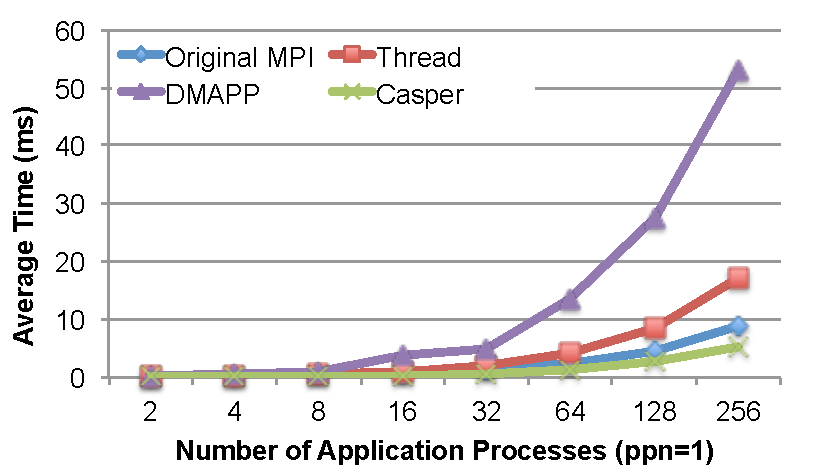
\includegraphics[width=0.64\columnwidth]{figures/casper/eva_cray_inter_np_1core.pdf}
  \label{fig:eva-scala-cray-acc}
}
\subfigure[Put on Cray XC30.]{
  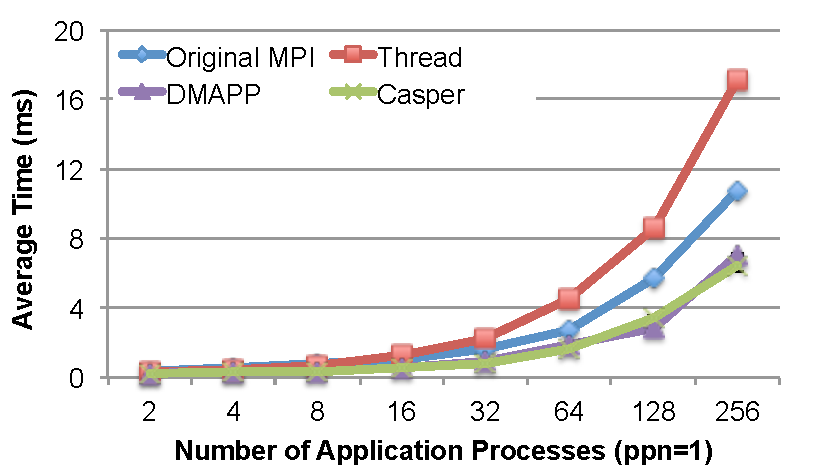
\includegraphics[width=0.64\columnwidth]{figures/casper/eva_cray_inter_np_1core_put.pdf}
  \label{fig:eva-inter-np-1core-put}
}
\subfigure[Accumulate on Fusion using MVAPICH.]{
  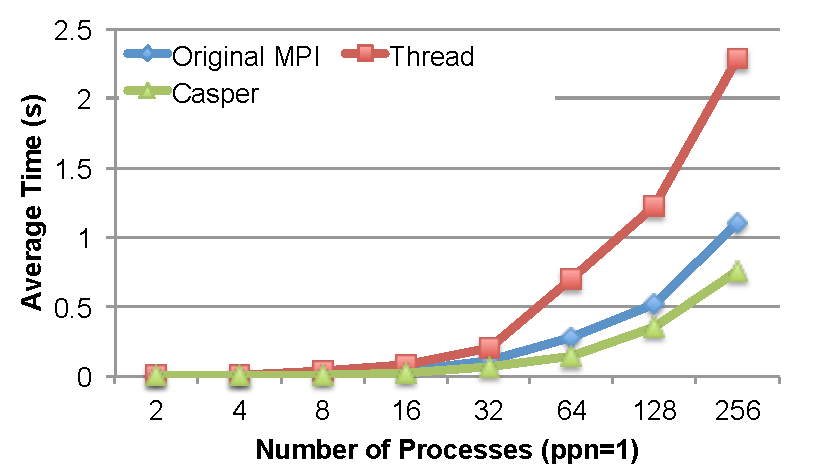
\includegraphics[width=0.64\columnwidth]{figures/casper/eva_fusion_inter_np_1core.pdf}
  \label{fig:eva-fusion-acc}
}
% \subfigure[Put on IB cluster using MVAPICH.]{
%   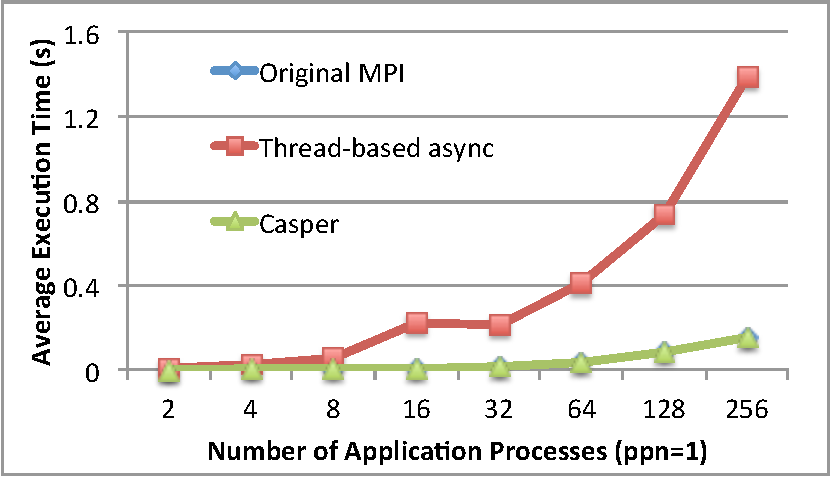
\includegraphics[width=0.48\columnwidth]{figures/casper/eva_fusion_inter_np_1core_put.pdf}
%   \label{fig:eva-fusion-put}
% }
% \subfigure[Accumulate in shared memory using MPICH.]{
%   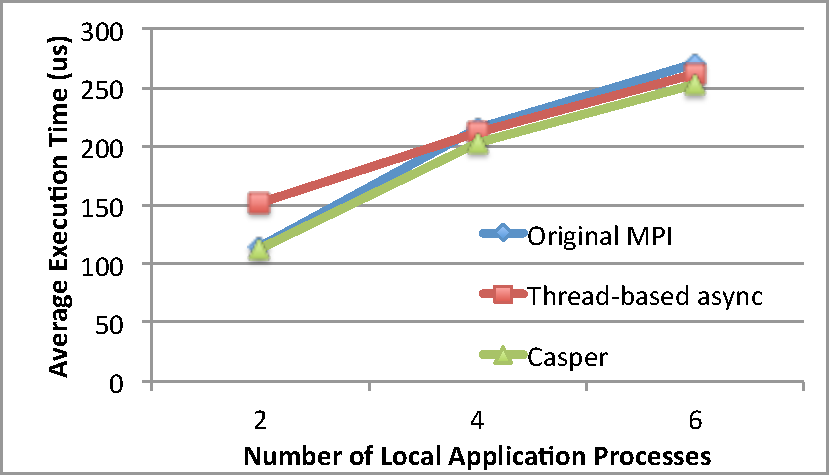
\includegraphics[width=0.62\columnwidth]{figures/casper/eva_mxm_async_acc.pdf}
%   \label{fig:eva-mxm-acc}
% }
% \subfigure[Lockall in shared memory using MPICH.]{
%   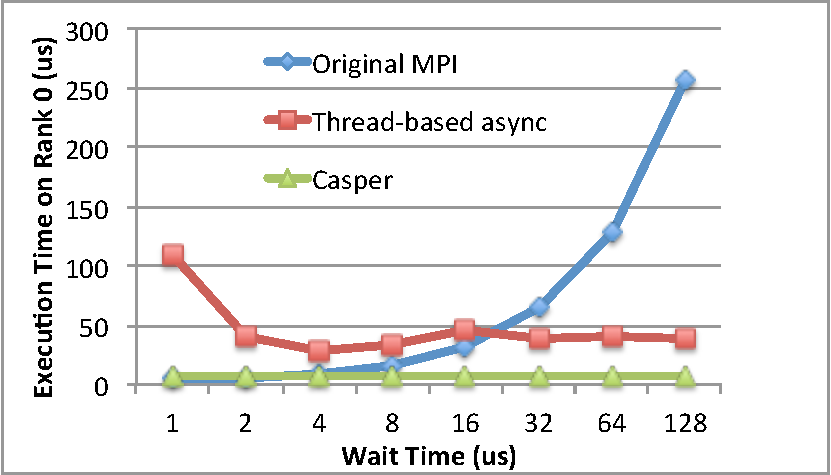
\includegraphics[width=0.62\columnwidth]{figures/casper/eva_mxm_async_lockall.pdf}
%   \label{fig:eva-mxm-lock}
% }
% \vspace{-1.0ex}
\caption{Asynchronous progress on different platforms.}
\label{fig:eva-scala}
% \vspace{-1.0ex}
\end{figure*}

% We also compared Casper with MPICH-SHM which supports direct RMA for
% all operations on shared memory.  Figure~\ref{fig:eva-mxm-acc} shows
% the performance of ACCUMULATE in the same
% \emph{communication--computation--communication} experiment described
% above.  It shows that Casper does not effect the performance of direct
% RMA operations on shared memory either.  However, although RMA
% operations are performed as direct RMA on shared memory,
% passive-target synchronization calls, such as \emph{lockall}, may
% internally involve two-sided communication which requires remote
% process to poll MPI progress.  We evaluate the asynchronous progress
% of \emph{lockall} on shared memory by measuring a test in which rank 0
% performs \emph{lockall--one accumulate--unlockall} to all the other
% local processes, and the others are busy computing.
% Figure~\ref{fig:eva-mxm-lock} shows the results using 6 processes on a
% single node.  As expected, with increasing computation on the target,
% the origin takes an increasing amount of time to finish its
% communication with original MPI.  Although both the asynchronous
% thread and Casper resolve this issue, the thread approach shows more
% overhead when the number of idle cores is not sufficient for running
% these per-process threads and results in core oversubscription (we run
% 6 processes on a 8 cores node).  Moreover, we notice that the thread
% asynchronous threads produce more overhead when the main thread of the
% waiting process only waits for 1 or 2~$\mu$s before entering into MPI
% stack and hence results in frequent lock contention.


%%%%%%%%%%%%%%%%%%%%%%%%%%%%%%%%%%%%%%%%%%%%%%%%%%%%
\subsection{Performance Optimization}\label{sec:eva-load}
%%%%%%%%%%%%%%%%%%%%%%%%%%%%%%%%%%%%%%%%%%%%%%%%%%%%

Our third set of microbenchmarks focuses on the different load-balancing
optimizations discussed in Section~\ref{sec:multi-ghost}.

%%%%%%%%%%%%%%%%%%%%%%%%%%%%%%%%%%%%%%%%%%%%%%%%%%%%
\subsubsection{Static Rank Binding}\label{sec:eva-static-rank}
%%%%%%%%%%%%%%%%%%%%%%%%%%%%%%%%%%%%%%%%%%%%%%%%%%%%

Figure~\ref{fig:eva-sta-load} shows our measurements with static rank
binding on Cray X30.  In the first experiment
(Figure~\ref{fig:eva-cray-sta-load-rank-nnp}) we show the static rank
binding with increasing number of processes when each process sends one
accumulate message (size of double) to every other process in the
system.  We use 16 processes per node and evaluate Casper with up to 8
ghost processes on each node.
Our results indicate that two ghost processes are sufficient
when up to 32 processes communicate; when more processes
communicate, however, configurations with larger numbers of ghost processes tend
to perform better.
The reason is that the number of
incoming RMA operations increases with more processes, thus requiring
more ghost processes computing to keep up.

Figure~\ref{fig:eva-cray-sta-load-rank-nop} shows a similar
experiment but increases the number of accumulate operations while
keeping the user process count constant at 32 (2 nodes with 16
processes each).  The results show a trend similar to that of the previous
experiment, with more ghost processes benefiting when the number of
operations per process is larger than 8.

%%%%%%%%%%%%%%%%%%%%%%%%%%%%%%%%%%%%%%%%%%%%%%%%%%%%
\subsubsection{Static Segment Binding}\label{sec:eva-static-seg}
%%%%%%%%%%%%%%%%%%%%%%%%%%%%%%%%%%%%%%%%%%%%%%%%%%%%

In this experiment we evaluate the performance of the static segment binding approach.  Such an approach is expected to be especially
beneficial when the application allocates uneven-sized windows and
receives a large number of operations that need to be processed in
software.  Figure~\ref{fig:eva-cray-sta-load-seg} demonstrates this
pattern.  We used 16 nodes with 16 processes and up to 8 ghost
processes per node.  The first
process of every node allocates a 4-kilobyte window (512 count of
double), while the others only allocate 16~bytes.  Then each process
performs a \emph{lockall--accumulate--unlockall} pattern on all the
other processes.  We increase the number of ACCUMULATEs to each
process whose local rank is 0 while issuing a single operation to
other processes.  As shown in the figure, performance improves with
increasing numbers of ghosts, because the large window is divided into
more segments and the communication issued to different segments is
handled by different ghosts.

\begin{figure*}
\centering
\subfigure[Static Rank Binding: Increasing Processes.]{
  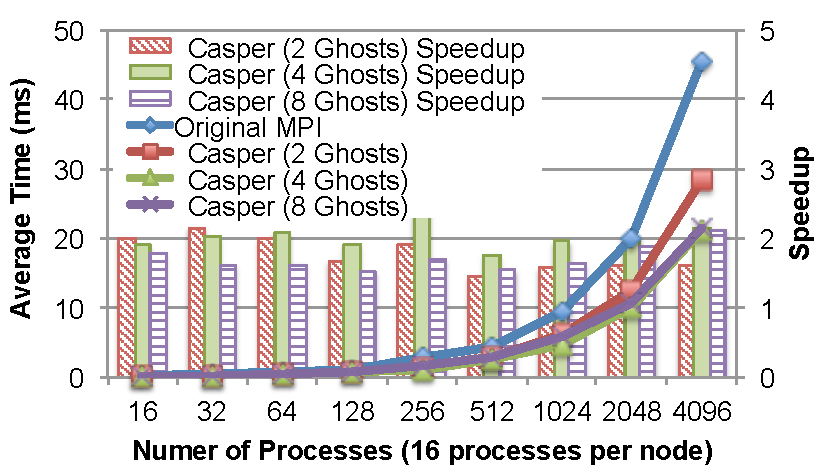
\includegraphics[width=0.64\columnwidth]{figures/casper/eva_cray_static_load_nnp.pdf}
  \label{fig:eva-cray-sta-load-rank-nnp}
}
\subfigure[Static Rank Binding: Increasing operations.]{
  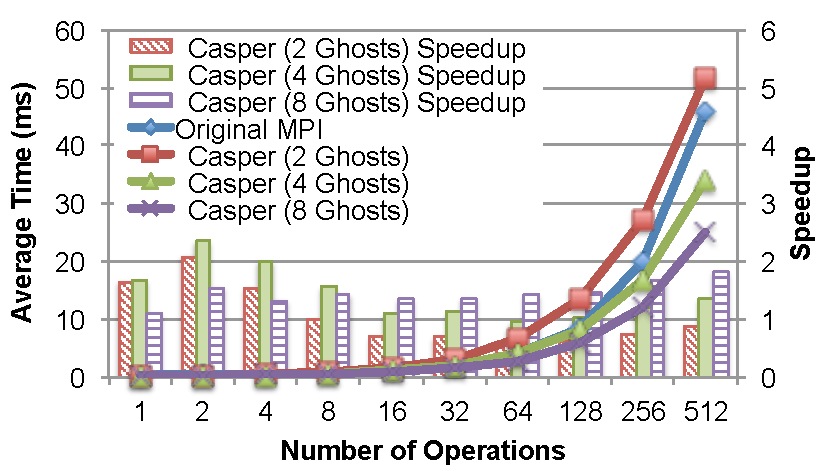
\includegraphics[width=0.64\columnwidth]{figures/casper/eva_cray_static_load_nop.pdf}
  \label{fig:eva-cray-sta-load-rank-nop}
}
\subfigure[Static Segment Binding: Uneven Window Size]{
  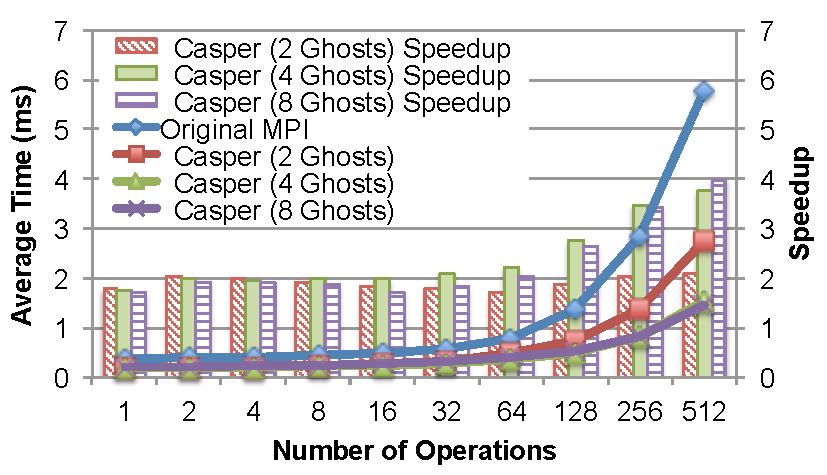
\includegraphics[width=0.64\columnwidth]{figures/casper/eva_cray_static_load_nseg.pdf}
  \label{fig:eva-cray-sta-load-seg}
}
% \vspace{-1.0ex}
\caption{Load balancing in static binding on Cray XC30.}
\label{fig:eva-sta-load}
% \vspace{-2.0ex}
\end{figure*}


%%%%%%%%%%%%%%%%%%%%%%%%%%%%%%%%%%%%%%%%%%%%%%%%%%%%
\subsubsection{Dynamic Binding}\label{sec:eva-dynamic-bind}
%%%%%%%%%%%%%%%%%%%%%%%%%%%%%%%%%%%%%%%%%%%%%%%%%%%%

To test our dynamic binding
approaches, we designed three microbenchmarks, all of which are
executed on 16 nodes with 20 user processes and 4 ghost processes per
node.

Figure~\ref{fig:eva-cray-runtime-load-random} shows the results of an experiment
in which all processes perform a \emph{lockall--put--unlockall} pattern
to all the other processes, but only the first rank of each node
receives an increasing number of PUT operations (varied on the x-axis
of the graph), while the others receive only one PUT operation.  Our
random load balancing simply chooses the ghost processes in the order
of its local rank for each target process.  Thus, all the PUT
operations are always equally distributed to the ghosts on each node
achieving much better performance that with static binding.

Figure~\ref{fig:eva-cray-runtime-load-op} uses a variant of the
previous experiment in which each process performs an uneven
\emph{lockall--accumulate--put--unlockall} pattern to all other
processes. In this case, random load balancing arbitrarily picks the
ghost process for each PUT operation but sends all ACCUMULATE
operations to the same ghost process (in order to maintain ordering
and atomicity guarantees).  Thus, the ghost process that is handling
both ACCUMULATE and PUT operations would end up having to handle more
operations than would the other ghost processes.  Our
``operation-counting'' approach, on the other hand, keeps track of
which ghost process has been issued how many operations and balances
the operations appropriately, thus allowing it to achieve better
performance than the random approach does.

Our third experiment,
uses yet another variant of the previous experiments by varying the
size of the operations while keeping the number of operations
constant.  Each process performs a
\emph{lockall--accumulate--put--unlockall} pattern, but only the
processes whose local rank is 0 receive increasing sizes of PUTs and
ACCUMULATEs (varied on the x-axis), while the others receive only one
double PUT and accumulate.
Figure~\ref{fig:eva-cray-runtime-load-byte} shows the results.
As expected, neither random nor
operation-counting algorithms can handle this case well, although
our ``byte-counting'' approach outperforms both of them.

\begin{figure*}
\centering
\subfigure[Random: Uneven Number of Put.]{
  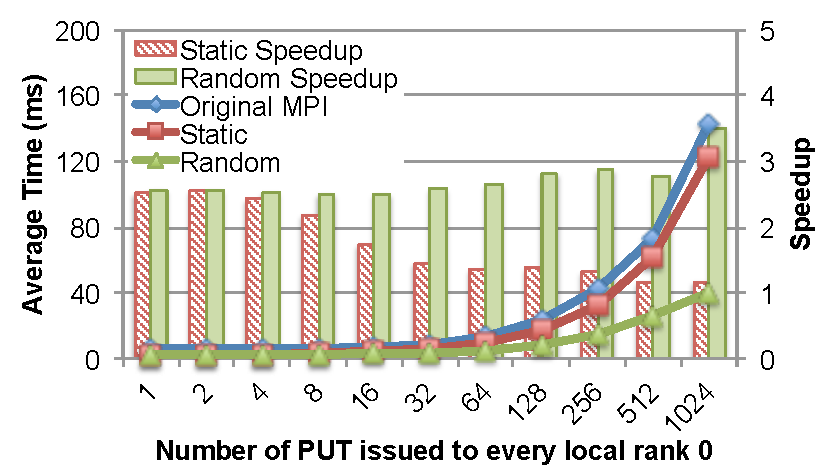
\includegraphics[width=0.64\columnwidth]{figures/casper/eva_cray_runtime_load_random.pdf}
  \label{fig:eva-cray-runtime-load-random}
}
\subfigure[OP-counting: Uneven Number of Put/ACC.]{
  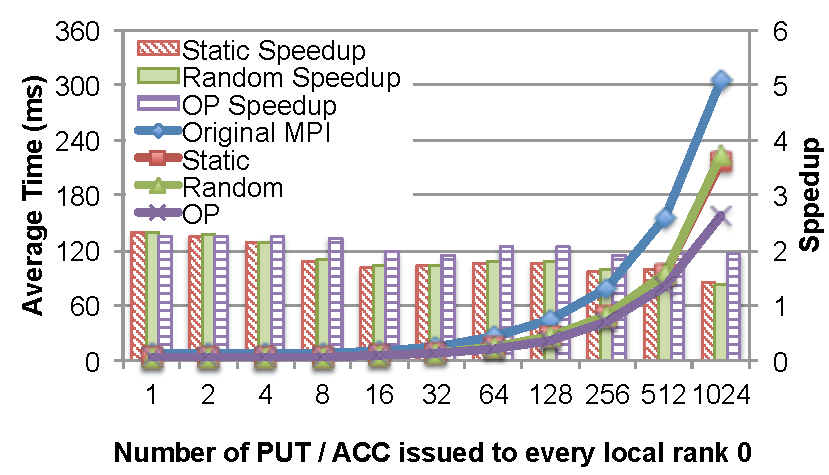
\includegraphics[width=0.64\columnwidth]{figures/casper/eva_cray_runtime_load_op.pdf}
  \label{fig:eva-cray-runtime-load-op}
}
\subfigure[Byte-counting: Uneven Size of Put/ACC.]{
  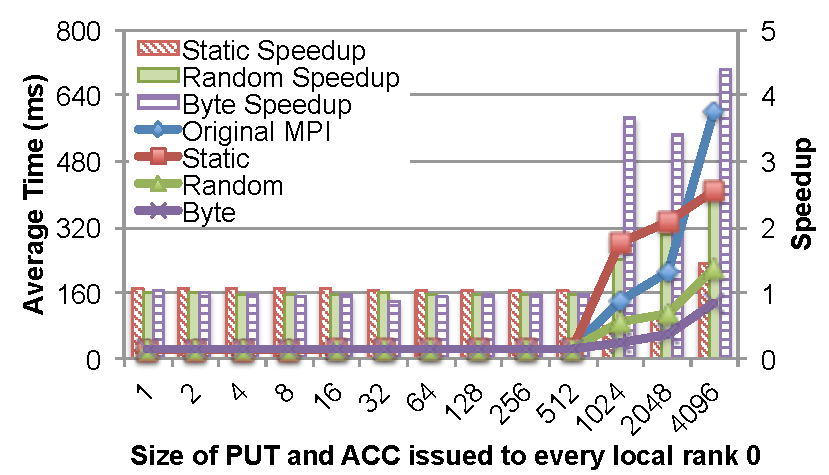
\includegraphics[width=0.64\columnwidth]{figures/casper/eva_cray_runtime_load_byte.pdf}
  \label{fig:eva-cray-runtime-load-byte}
}
% \vspace{-1.0ex}
\caption{Dynamic load balancing on Cray XC30.}
\label{fig:eva-runtime-load}
% \vspace{-4.0ex}
\end{figure*}

% %%%%%%%%%%%%%%%%%%%%%%%%%%%%%%%%%%%%%%%%%%%%%%%%%%%%
% \subsubsection{Memory Locality Comparison}\label{sec:eva-locality}
% %%%%%%%%%%%%%%%%%%%%%%%%%%%%%%%%%%%%%%%%%%%%%%%%%%%%
% The last microbenchmark measures the overhead when
% ghost process is located in a different NUMA domain with
% the application process. We simply use two interconnected processes
% each with a ghost process on its node, one process issues
% \emph{lock-100 accumulate-unlock} to the second process while
% the second one waits in MPI barrier. Figure~\ref{fig:eva-cray-locality}
% shows that significant overhead occurs on Cray XC30 when the ghost
% process is located in a different NUMA domain and accesses the
% memory of application process across domain. The overhead
% even increases with increasing size of operations, 120\% overhead
% is produced when issuing 512 could of double(4097~Bytes) operation .

% \begin{figure}[h]
% \centering
% 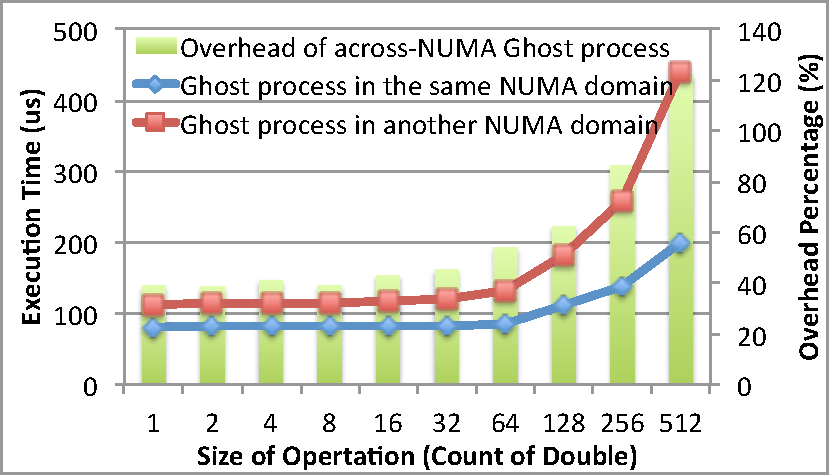
\includegraphics[width=0.8\columnwidth]{figures/casper/eva_edison_locality.pdf}
% \caption{Comparison of two cases with different ghost process location.}
% \label{fig:eva-cray-locality}
% \end{figure}




%%%%%%%%%%%%%%%%%%%%%%%%%%%%%%%%%%%%%%%%%%%%%%%%%%%%
\subsection{NWChem Quantum Chemistry Application}\label{sec:eva-realapp}
%%%%%%%%%%%%%%%%%%%%%%%%%%%%%%%%%%%%%%%%%%%%%%%%%%%%

NWChem~\cite{NWChem63} is a computational chemistry application suite
offering many simulation capabilities.  For massively
parallel simulations, a common method employed is coupled-cluster
theory (CC), for which NWChem has extensive
functionality~\cite{Hirata:2003:JPCA:TCE} and excellent
performance~\cite{Apra:2009:SC:NWChem}.  For data movement, NWChem uses the Global
Arrays~\cite{GA_SC94} toolkit, which has been
implemented on a number of platforms natively and as a portable
implementation over MPI RMA~\cite{dinan12:armci_mpi}.

Because CC simulations are one of the most common usages of NWChem in
the context of large clusters or supercomputers, our experiments focus
on the most popular CC method, CCSD(T).
Two molecules are considered: the water cluster (H$_2$O)$_n$
($n=16$)---denoted W$n$ for short---and C$_{20}$, obtained
from the NWChem QA test suite (\texttt{QA/tests/tce\_c20\_triplet}).
For the water cluster, we used double-zeta basis sets (cc-pVDZ from
the NWChem basis set library), which are reasonable for this class of
problems.  We compared Casper with both the original MPI and two
thread-based approaches.
The first approach employs oversubscribed cores
(Thread~(O)), where every thread and its MPI process execute on
the same core; the second approach uses dedicated cores (Thread~(D)),
where threads and MPI processes are on separate cores. We used the same total
number of cores in all approaches, some of which are dedicated to
asynchronous ghost processes\slash threads as listed in Table~\ref{tab:eva-nwcore}.

\begin{table}\scriptsize
\begin{center}
\caption{Core deployment in NWChem evaluation on Cray XC30.}\label{tab:eva-nwcore}
\begin{tabular}{|c|c|c|}
\hline
& Computing Cores & Async Cores \\
\hline
Original MPI & 24 & 0 \\
Casper & 20 & 4 \\
Thread (O) & 24 & 24 \\
Thread (D) & 12 & 12 \\
\hline
\end{tabular}
\end{center}
% \vspace{-4.0ex}
\end{table}

Figures~\ref{fig:eva-edison-nw-w16} and
\ref{fig:eva-edison-nw-c20-ccsd} report timings for a single
iteration of CCSD, which is a communication-intensive solver composed
of more than a dozen tensor contractions of varying size.  For smaller
problems, when computation dominates, asynchronous progress is more
important because the application is calling MPI relatively
infrequently.  At larger scale, the computation time decreases, and the
communication is more frequent; hence the improvement with Casper is
less.  The (T) portion of the CCSD(T) methods is much more
compute-intensive. Hence, the time between MPI calls can be
large, and thus the impact of asynchronous progress is
significant.  Each process fetches remote data, then does significant
computation---over and over. As a result, the lack of progress causes
processes to stall, waiting on GET operations to be satisfied remotely.
Figure~\ref{fig:eva-edison-nw-c20-ccsdt} shows the significance of
asynchronous progress at all scales.  Relative to the original
version, Casper is almost twice as fast; but thread-based asynchronous
progress is far less effective. The reason is that although both approaches
improve asynchronous progress in communication, the thread-based
solutions significantly degrade the performance of computation, either by
core oversubscription or by appropriation of half of the computing cores.

\begin{figure*}
\centering
\subfigure[CCSD for W16=(H$_2$O)$_{16}$ with pVDZ]{
  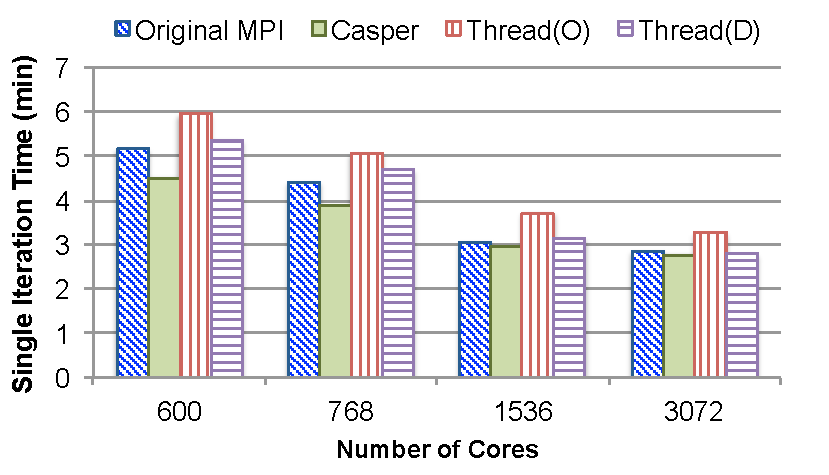
\includegraphics[width=0.64\columnwidth]{figures/casper/eva_edison_nwchem_w16_dz.pdf}
  \label{fig:eva-edison-nw-w16}
}
\subfigure[CCSD for C$_{20}$ with pVTZ]{
  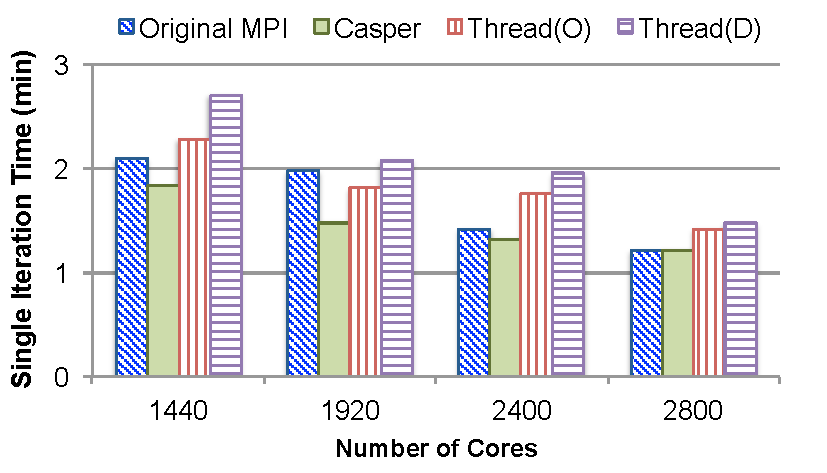
\includegraphics[width=0.64\columnwidth]{figures/casper/eva_edison_nwchem_tce_c20_ccsd.pdf}
  \label{fig:eva-edison-nw-c20-ccsd}
}
\subfigure[(T) portion of CCSD(T) for C$_{20}$ with pVTZ]{
  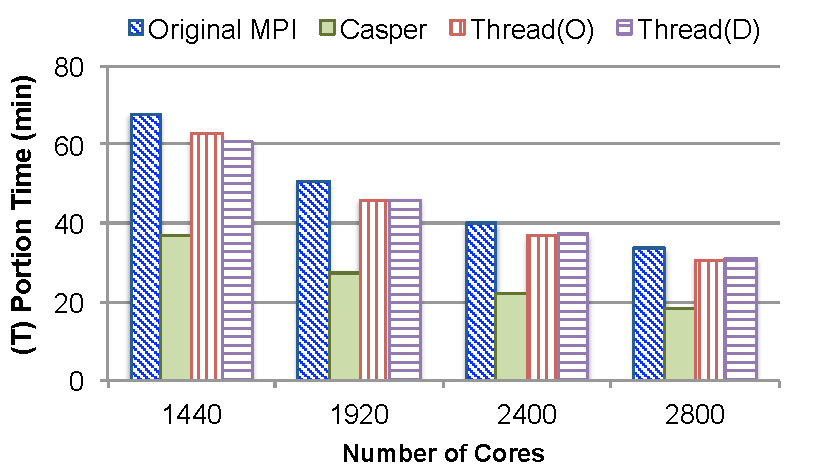
\includegraphics[width=0.64\columnwidth]{figures/casper/eva_edison_nwchem_tce_c20_ccsdt.pdf}
  \label{fig:eva-edison-nw-c20-ccsdt}
}
% \vspace{-1.0ex}
\caption{NWChem TCE coupled cluster methods on Cray XC30.}
\label{fig:eva-nwchem}
% \vspace{-4.0ex}
\end{figure*}


